
\section*{2.3 Cart-Pole Balance}

\subsection*{2.3(a)}
With \(\tilde s_k=s_k-\bar s\), Euler discretization gives
\[
    \tilde s_{k+1}\approx A\tilde s_k+Bu_k,
\]
where
\[
    A=I+\Delta t
    \begin{bmatrix}
    0&0&1&0\\
    0&0&0&1\\
    0&\frac{m_pg}{m_c}&0&0\\
    0&\frac{(m_c+m_p)g}{m_c\ell}&0&0
    \end{bmatrix},
    \qquad
    B=\Delta t
    \begin{bmatrix}
    0\\0\\ \frac{1}{m_c}\\ \frac{1}{m_c\ell}
    \end{bmatrix}.
\]

\subsection*{2.3(b)}
Using Riccati recursion until
\(\|P_k-P_{k-1}\|_{\max}<10^{-4}\) gives
\[
    \boxed{K_\infty=
    \begin{bmatrix}
    0.73&-231.85&4.22&-68.25
    \end{bmatrix}.}
\]

% \subsection*{2.3(c)}
% \begin{figure}[H]
% \centering
% 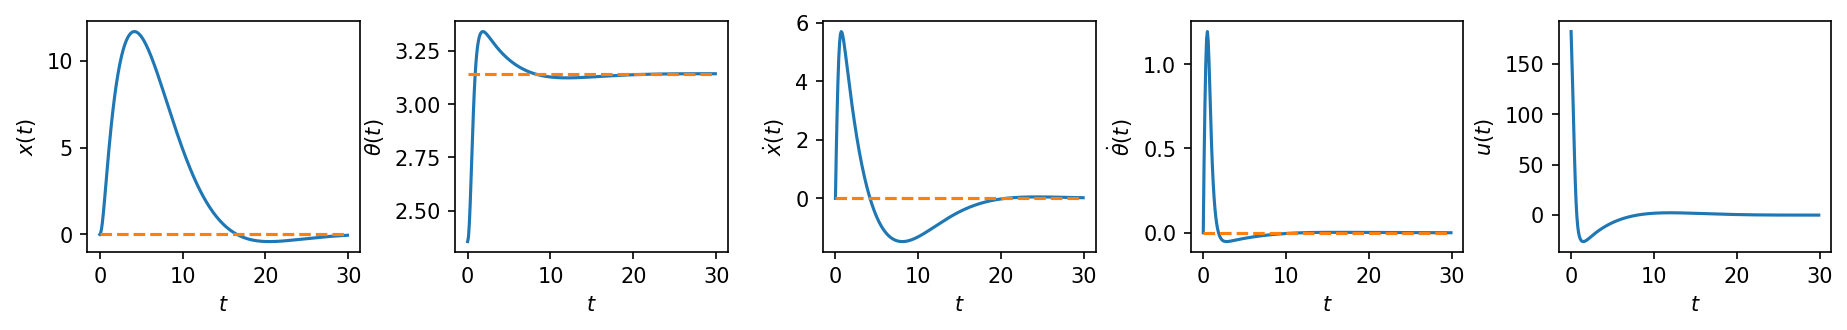
\includegraphics[width=\textwidth]{figures/cartpole_balance.png}
% \caption{Cart-pole balance with the infinite-horizon LQR controller.}
% \end{figure}

\subsection*{2.3(d)}
\textbf{i.} We can reuse \(A\) and \(B\) because the dynamics Jacobians along
the reference do not depend on \(x\), and the desired trajectory keeps
\(\theta=\pi\), \(\dot\theta=0\). Therefore the same upright linearization is
valid along the reference.

% \textbf{ii.}
% \begin{figure}[H]
% \centering
% 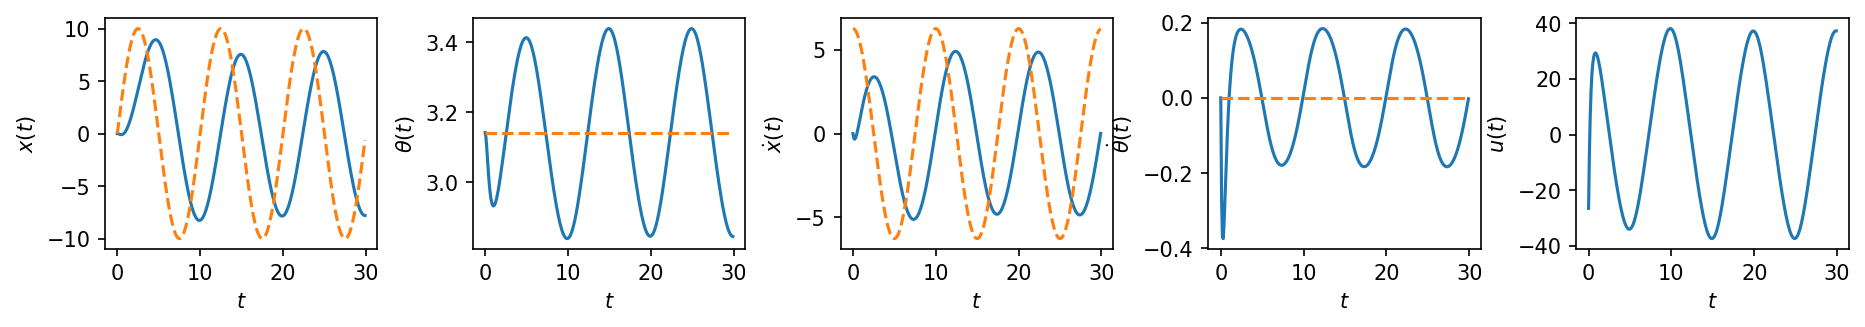
\includegraphics[width=\textwidth]{figures/cartpole_balance_tv.png}
% \caption{Tracking \(x_{\rm ref}(t)=10\sin(2\pi t/10)\) with LQR feedback.}
% \end{figure}

\textbf{iii.} The reference cart motion has nonzero acceleration, but the
reference does not include a dynamically consistent feedforward force. The
pendulum must tilt to generate the horizontal cart acceleration, so keeping
\(\theta(t)\equiv\pi\) while moving the cart sinusoidally is not a dynamically
consistent upright trajectory without feedforward compensation.
